\begin{frame}
    \frametitle{Equilibrium with no Runs}

    \setcounter{theorem}{1}

    \begin{lemma}
        In equilibrium, all commercial banks that have depositors 
        make zero-profis and offer socially optimal contract.
    \end{lemma}

    \begin{lemma}
        The foreign CB can replicate the socially optimal bank deposit contract, 
        if $c^*_1 = \bar{c}_1$ and $c^*_2 = \bar{c}_2$
    \end{lemma}

    \begin{proposition}
        In an equilibrium, 
        \begin{enumerate}
            \item DB offers better contract : $f=0$
            \item FCB offers better contract : $f=k$
            \item Both offer best : $f\in(0,k)$
        \end{enumerate}
    \end{proposition}
\end{frame}

\begin{frame}
    Denote the social optimal contract and short-term investment as a tuple 
    $(\bar{c}_1, \bar{c}_2, \bar{y})$. 

    The payoff matrix for an early withdraw episode:
    \renewcommand{\arraystretch}{3}
    \begin{table}
        \begin{tabular}{c|c|c}

            Event   & Withdraw & Roll-over \\
            \hline
            No run & $u(\bar{c}_1)$ & $u \left(\frac{R[(1-\bar{y}) - (\alpha - \lambda)\bar{c}_1 / l]}{1-\alpha}\right)$ \\
            Run & $\frac{r\bar{y} + (1-y)l}{\alpha \bar{c}_1} u(\bar{c}_1)$ & $0$ \\
            
        \end{tabular}
    \end{table}

    Strategic complementarity.
    \renewcommand{\arraystretch}{1}
\end{frame}

\begin{frame}
    \frametitle{Equilibrium with Runs in the Foreign CBDC}

    \setcounter{theorem}{5}
    \begin{lemma}
        If the foreign central bank offers a riskless deposit contract which 
        mimics the payoff of the social-optimal contract, then it will attract all deposits 
        up to the capital account constraint.
    \end{lemma}

    \begin{alertblock}{Point of view}
        \begin{enumerate}
            \item Lack of proper proof. At least model an exogenous probability of run to justify the lemma.
            \item Too strong an assumption; deposits are also used as digital payment assets, 
                    it is too naive to discard the fact that an asset can be MoP.
        \end{enumerate}
        
    \end{alertblock}

\end{frame}

\begin{frame}
    \frametitle{Non-social optimal contract for F-CBDC}

    \begin{proposition}
        As consumers internalize that the foreign central bank deposit contract is perfectly safe, 
        the foreign central bank can offer a deposit contract with lower payoffs than the social optimal one, 
        and still attract the highest possible amount of deposits (up to the capital account constraint).
    \end{proposition}

    The author's ``proof'' : 

    As run can occur with commercial banks, but not with central bank, 
    it has to be that $U_1 < U_2$

\end{frame}

\begin{frame}[plain]

    \begin{figure}
        \centering
        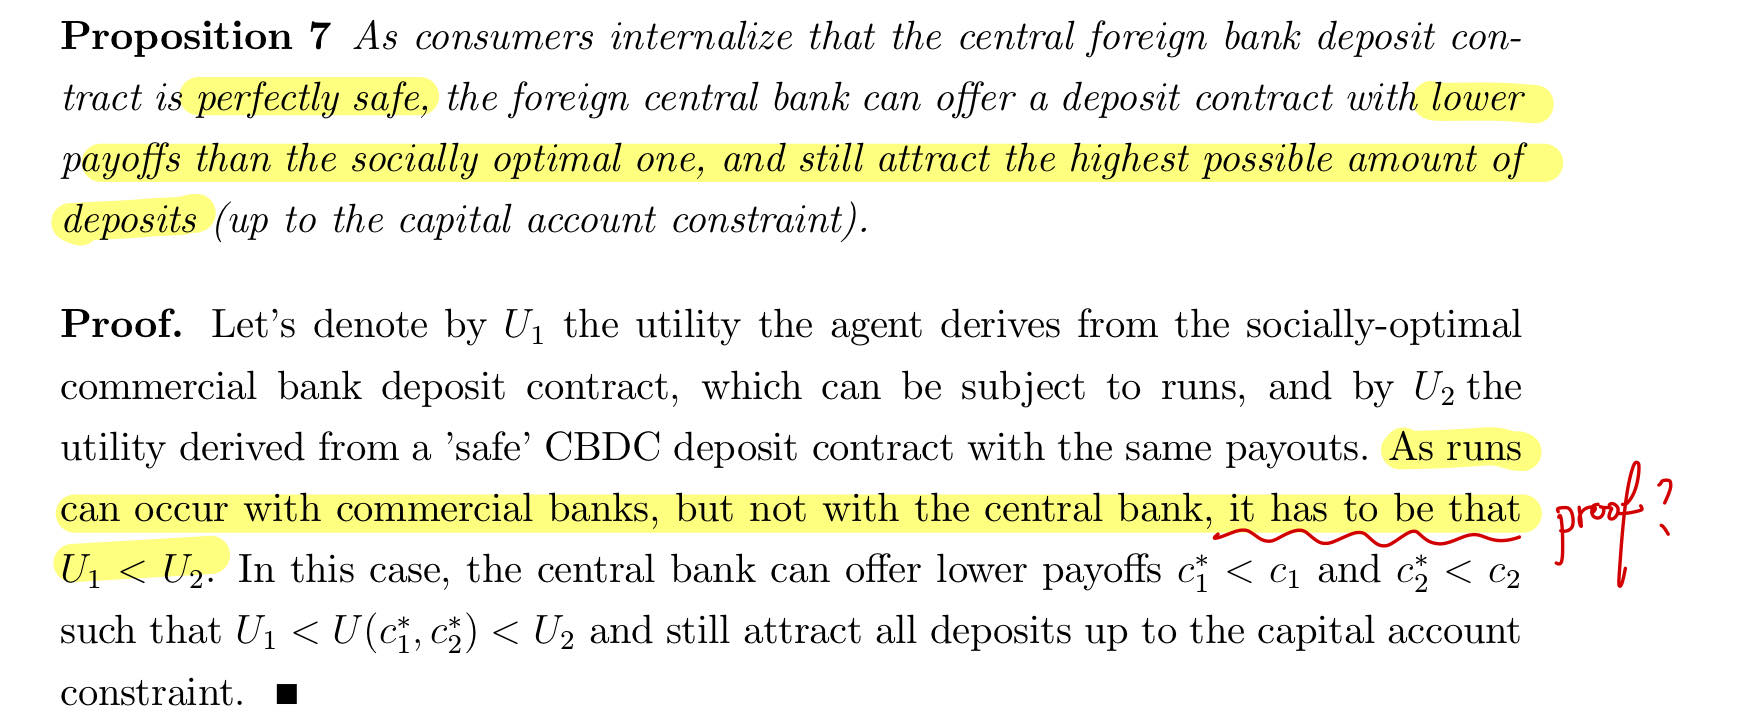
\includegraphics[width = \textwidth]{fig/wtf.jpg}
    \end{figure}
\end{frame}